\chapter{脑电电势准确性的参考等多因素研究}
\section{研究背景}
不当参考导致的波形失真对定量脑电分析的影响是全局性的,参考选择是脑电数据处理的基础关键环节。本章旨在系统研究参考模态和电极配置对脑电电位的准确性影响。脑电的成功应用取决于信号处理方法如时域信号的时频分析\citing{koenig_t_topographic_2001},头表空间地形图分析\citing{lehmann_d_multichannel_1971,lehmann_d_eeg_2009},以及大脑源空间的层析成像分析\citing{rd_pascual-marqui_review_1999,grech_r_review_2008,valdes_p_frequency_1992}。这些都要求对源模型\citing{scherg_m_fundamentals_1990}、头模型、容积传导模型的准确估计或模拟,但最重要的是获取更加准确的脑电电势。

为获取准确脑电电势不仅要控制各种环境噪声还要降低非中立零参考的失真效应。脑电电势是活跃电极与参考电极\citing{nunez_p_l_eeg_1997}间的电势差。过去几十年,人们一直在追求近似的零参考,以便活跃电极能通过某参考电极准确记录到时变电势。然而,在身体表面不可能找到不活跃中立的参考位点。参考选择不但没得到较好解决还形成不一致的用法和无休止的争论,这就是所谓的\textit{参考电极问题}。目前已有多种参考模态,包括在线记录参考(常用的各种单极参考)和几种离线重参考如连接耳参考(LM)\citing{garneski_t_m_and_steelman_h_f_equalizing_1958}、平均参考(AR)\citing{offner_eeg_1950}和零参考(REST)\citing{yao_method_2001}。研究表明参考选择对脑电波形和功率谱有显著影响\citing{zhai_y_and_yao_d_study_2004,
rellecke_j_emotion_2013,chella_f_non-linear_2017},参考的效果受到各种因素特别是电极数的影响\citing{yao_method_2001,liu_q_estimating_2015,lei_x_and_liao_k_understanding_2017,chella_impact_2016}。

当前实际应用中电极数参差不齐变动范围很大:临床中常用10导联或16导联,认知神经科学研究中常采用64-256导联的高密度阵列,一些研究甚至用到多于300导联的超高维阵列\citing{oostenveld_r_and_praamstra_p_five_2001,jurcak_v_1020_2007}。然而,以前关于电极导联数的研究局限于21-256导联。现在有必要对覆盖10导联到300导联以上的电极数进行综合比较研究。随着电极数增多电极具有不同分布规律。具有21电极数的国际10-20标准放置系统是标准化电极分布的第一份报告\citing{jasper_h_h_ten_1958}。 10-10和10-05系统是10-20系统的衍生,只是采用更多电极并加以命名以满足源成像技术的需要\citing{oostenveld_r_and_praamstra_p_five_2001,
jurcak_v_1020_2007,nuwer_m_r_ifcn_1998,chatrian_g_e_and_lettich_e_n_p_ten_1985}。这些系统在原来10-20系统的基础上按照相对等分头表位置准则定义更多的电极位置。本章称这一系列为10-x系统。另外一种分布由美国公司Electrical Geodesics, Inc.提出,思路是按照测地传感网络(GSN)放置更多电极,好似在球面上剖分多边形并指定多边形的中心作为电极位置\citing{tucker_d_m_spatial_1993},便于高密度成像\citing{michel_c_m_and_lantz_g_getting_2004}。本章称这种电极分布为GSN系统。这两种分布的区别在于电极是否覆盖面颊和颈部。不同电极分布条件下参考选择对矫正电位失真的效果差异一直是被忽视的问题。

本章研究参考模态和电极配置两个关键因素。首先用源空间中单个偶极子源正演计算得到标准脑电电位。通过正演计算得到电位的参考是理想无穷远参考,这是正演理论内在决定的。然后标准脑电电位被转换到具有不同参考的记录,包括五种单极参考(左耳垂、Fz、Pz、Oz、Cz)和三种重参考(LM、AR和REST)。最后标准脑电电位和转换的某参考脑电电位间的相对误差被关于多种因素进行比较,例如电极数、头表电极位置区域、电极分布、偶极子源位置方向以及电极测量噪声和头模型等。研究发现在线记录参考通常扭曲脑电电位波形,需要用重参考矫正这种失真效应。重参考中,REST对各种因素具有比AR更好的效果,LM最差,AR的效果受到电极分布及偶极子方向的制约但与电极数无太大关系。这表明REST可作为脑电重参考的首选,电极噪声较大时AR可作为REST的替代选择。

\section{仿真方法}
\begin{figure}[!ht]
	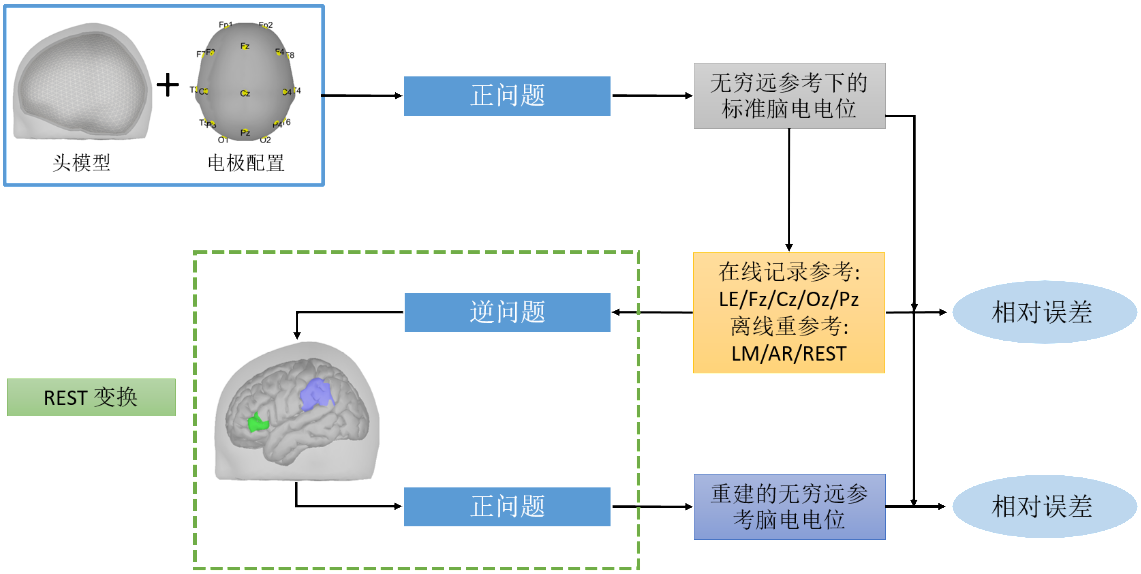
\includegraphics[width=15cm]{pic/JNE/figure1.png}
	\caption{标准脑电电位生成、参考转换、误差分析流程图。给定头模型和电极配置,正演生成无穷远参考电位作为基标准,标准电位被转换为不同
	参考的记录。最后交叉比较参考模态、电极配置和其他因素条件下转换参考电位与基准电位的相对误差。}
	\label{2:pipe}
\end{figure}
仿真分析流程如图\ref{2:pipe}所示,首先构造两个三层头模型,分别具有同心球和真实头形状。假设偶极子源分布在皮层表面及大脑三维容积栅格中。电极按10-x或GSN分布并配准在大脑头皮表面。然后通过正演公式仿真基于无穷远参考的标准电位并进一步转换为五种单极参考记录 (如左耳(LE)、Fz、Cz、Pz、Oz) 和三种重参考记录(LM、AR、REST)。最优的参考模态和电极配置就是离标准电位偏差最小的情况。

三层头模型包括大脑皮层、颅骨、头皮,相对容积传导率分别为1、0.0125、1。对于同心球头形状\citing{yao_method_2001,yao_d_high-resolution_2000},头表面、颅骨内外表面的相对半径分别是1.0、0.87、0.92。源空间由均匀径向垂直分布于大脑皮层(半径=0.86)的2600个离散偶极子和均匀分布在皮层下区域的三维栅格中(半径$\leq$0.84)1269*3正交偶极子构成。同心球面头模型的偶极子总数达到6407。基于MNI结构磁共振数据模板ICBM152\citing{fonov_v_unbiased_2009,fonov_v_unbiased_2011}估计出真实头模型。配准电极到头表后用OpenMEEG\citing{gramfort_a_forward_2011}和Brainstorm\citing{tadel_f_brainstorm_2011,symond_m_p_gamma_2005}中的边界元法\citing{kybic_j_common_2005}正演计算头表电位。头表面、颅骨内外三层表面的每层均由1922顶点组成,颅骨厚度为4mm。源空间由所有皮层顶点上的15002*3正交偶极子组成。因此,真实头模型中共考虑45006个偶极子。

\subsection{标准脑电电位生成}
给定头模型和电极坐标可以计算出传递矩阵$\mathbf{K}\in{\mathbb{R}^{N_e\times{N_s}}}$。已知单个时刻点所有偶极子源活动强度$\mathbf{j}$,根据麦克斯韦方程的准静态估计\citing{gulrajani_bioelectricity_1998},所有电极的脑电电位可通过如下公式得到
\begin{equation}\label{eq2.1}
\mathbf{v}_{\infty}=\mathbf{Kj}
\end{equation}
这里传递矩阵$\mathbf{K}$是基于无穷远参考\citing{de_munck_j_c_potential_1988,wolters_c_h_efficient_2004}。源活动和多通道电位间的关联协同是基于无穷远处的中立零参考。脑电正演模型是所有偶极子源活动单个时刻点的线性组合。给定头模型和电极配置,脑电电位由相同时刻点下的源活动决定。参考问题源自偶极子源活动几乎瞬间同时到达活跃电极和参考点,本章仅考虑单个时刻点。为减小特定源位置造成的偏差依次检测偶极子正演电位参考前后的误差。共对电极数$N_e$乘源个数$N_s$的标准脑电电位进行误差估计。由于\eqref{eq2.1}的线性可以相似地评价不同源活动任意组合条件下参考前后误差。
\subsection{传感器电极噪声测试}
实际记录的脑电信号中不可避免地引入电极测量噪声。噪声可能产生于各种未知的源,采用零均值多变量高斯分布仿真电极测量噪声$\mathbf{\epsilon}$。因此\eqref{eq2.1}中脑电生成模型变为
\begin{equation}\label{eq2.2}
\begin{aligned}
\tilde{\mathbf{v}}_\infty& =\mathbf{v}_{\infty}+\mathbf{\epsilon},\mathbf{\epsilon}\sim{N(\mathbf{0},\mathbf{I}_{N_e})}\\
SNR& =10\log_{10}(\lVert{\mathbf{v}_\infty}\rVert_2^2/\Vert{\mathbf{\epsilon}}\rVert_2^2)
\end{aligned}
\end{equation}
这里,$\mathbf{0}\in{\mathbb{R}^{N_e\times1}}$,$\mathbf{I}_{N_e}\in{\mathbb{R}^{N_e\times{N_e}}}$是单位矩阵; SNR是无噪
声脑电信号$\mathbf{v}_{\infty}$与电极噪声$\mathbf{\epsilon}$的能量比例,单位为分贝dB;$\lVert{\cdot}\rVert_2^2$指的是$\ell_2$模的平方。
\subsection{电极数与分布系统}
这里研究11种电极数和2种电极分布,前后两者都可能影响脑电电位准确性。如图\ref{2:layout}所示,电极数10、16、21、32、64、85、96、128、335服从10-x分布,电极数129、257服从GSN电极分布。
关于电极标号和三维笛卡尔坐标,10、16和21通道的命名和坐标取自10-20电极分布\citing{jasper_h_h_ten_1958};32、64、96和128电极使用的10-10 c分布,取自ActiCHamp128Ch标准(Brain Products Co. Ltd,德国);129、257通道取自HydroCel™ Geodesic Sensor Net E001标准(Electrical Geodesics, Inc.,美国);64、85通道分别用的是10-10 n分布、10-10 r分布,335通道的坐标取自10-05系统\citing{oostenveld_r_and_praamstra_p_five_2001}。
\bigskip
\bigskip
\bigskip
\bigskip
\begin{figure}[!ht]
	\centering
	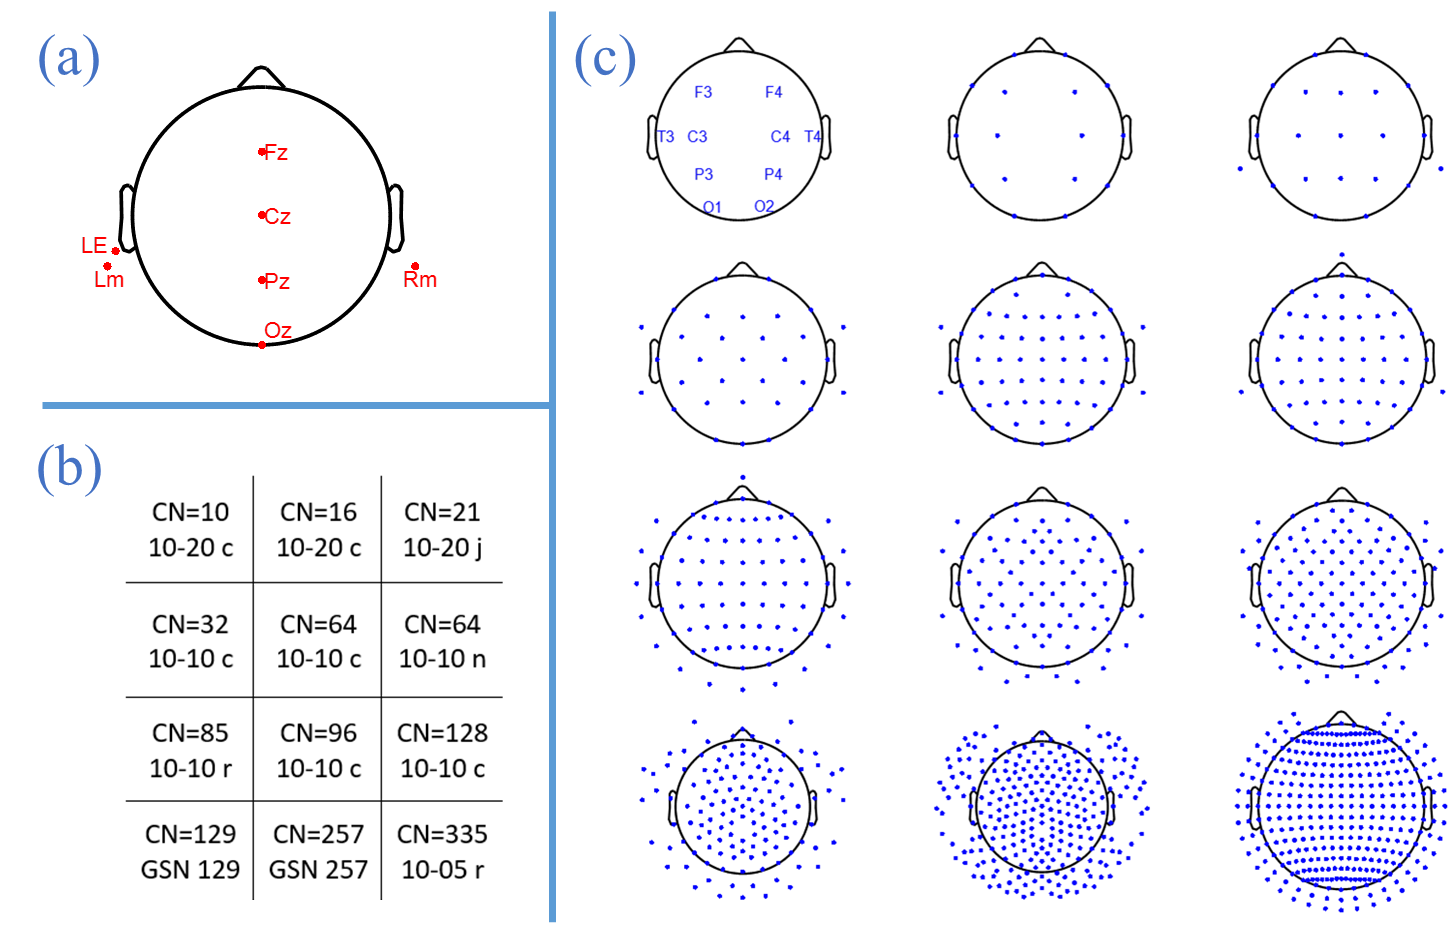
\includegraphics[width=15cm]{pic/JNE/figure2.png}
	\caption{电极配置策略。A.五种单极参考:LE、Fz、Pz、Oz、Cz和左右乳突(Lm, Rm);B.电极数(CN)和电极分布:10-20 c—临床使用的10-20系统;10-20 j—国际标准化10-20系统\citing{jasper_h_h_ten_1958};10-10 c—商业10-10系统(Brain Products Co. Ltd,德国);10-10 n—扩展\citing{nuwer_m_r_ifcn_1998}的标准10-10系统;10-10 r和10-05 r—论文\citing{oostenveld_r_and_praamstra_p_five_2001}定义的10-10和10-05系统;GSN 129/257—研究\citing{tucker_d_m_spatial_1993}提出的Geodesic Sensor Net多边形放置系统。C.电极分布地形图。}
	\label{2:layout}
\end{figure}
\subsection{几种参考转换方法}
所有的参考转换过程一般表示为
\begin{equation}\label{eq2.3}
\mathbf{v}_r=\mathbf{Tv}_{\infty}
\end{equation}
这里$\mathbf{v}_{\infty}$是无穷远参考下的脑电电位,$\mathbf{T}$是特定参考下的转换矩阵。 $\mathbf{v}_r$是转换为参考$r$时的脑电电
位。
\subsubsection{在线记录参考}
单极参考的原理是从所有活跃电极减去单极物理参考电极的电位,即
\begin{equation}\label{eq2.4}
\mathbf{T}=\mathbf{T}_{r},\quad\mathbf{T}_{r}=\mathbf{I}_{N_{e}}-\mathbf{1}\mathbf{f}^T,\quad\mathbf{f}=[0,...,1,...,0]^T
\end{equation}
这里$\mathbf{1}\in{\mathbb{R}^{N_e\times1}}$是单位向量,$\mathbf{f}\in{\mathbb{R}^{N_e\times1}}$是只有一个非零元1位于单极参
考对应行,可能是左侧耳垂LE、Fz、Pz、Oz和Cz其中之一。

\subsubsection{重参考技术}
重参考是进一步变换已使用某种参考测量的脑电电位,在线记录参考已经固有地参与其中。

连接耳参考 (LM)
\begin{equation}\label{eq2.5}
\mathbf{T}=(\mathbf{I}_{N_e}-\mathbf{1f}^T)\mathbf{T}_r,\quad\mathbf{f}=[0,...,0.5,...,0.5,...0]^T
\end{equation}
这里$\mathbf{f}$是仅具有两个非零元0.5位于左右乳突对应行的零向量。

平均参考 (AR)
\begin{equation}\label{eq2.6}
\mathbf{T}=(\mathbf{I}_{N_e}-\mathbf{1f}^T)\mathbf{T}_r,\quad\mathbf{f}=[1/{N_e},...,1/{N_e}]^T
\end{equation}
这里$\mathbf{f}$的所有元是$1/{N_e}$.

零参考(REST)
将等式\eqref{eq2.1}和\eqref{eq2.4}代入\eqref{eq2.3}得到$\mathbf{v}_r=\mathbf{T}_{r}\mathbf{Kj}$。根据等效偶极子源
理论\citing{yao_method_2001,yao_d_high-resolution_2000},头表电位$\mathbf{v}_{\infty}$由实际源$\mathbf{j}$通过传递矩阵$\mathbf{K}$生成,也可通过等效源$\mathbf{j}_1$和传递矩阵$\mathbf{K}_1$得到,即
\begin{equation}\label{eq2.7}
\mathbf{v}_{\infty}=\mathbf{Kj}=\mathbf{K}_1\mathbf{j}_1
\end{equation}
这里$\mathbf{j}_1$可能是分布在二维皮层薄片栅格上覆盖所有实际偶极子在内的等效源,或与实际源重叠的三维分布源,或是坐标系统原点上的多极源\citing{yao_d_high-resolution_2000}。 对于REST,尽管实际源$\mathbf{j}$和传递矩阵$\mathbf{K}$未知,可用假设的等效源$\mathbf{j}_1$和相应的传递矩阵$\mathbf{K}_1$\citing{yao_method_2001,zhai_y_and_yao_d_study_2004}。本章球面头模型和真实头模型分别用三维栅格上具有三正交方向的偶极子源和具有固定径向于皮层方向的皮层偶极子作为$\mathbf{j}_1$。因为脑电逆问题与参考无关\citing{pascual-marqui_r_d_and_lehamann_d_topographic_1993,geselowitz_d_b_zero_1998},$\mathbf{j}_1$的近似估计是
\begin{equation}\label{eq2.8}
\hat{\mathbf{j}}_1=(\mathbf{T}_r\mathbf{K}_1)^+\mathbf{v}_r
\end{equation}
代入公式\eqref{eq2.8}和\eqref{eq2.3}到\eqref{eq2.7},无穷远参考下的脑电电位$\mathbf{v}_{\infty}$可以近似重建为
\begin{equation}\label{eq2.9}
\mathbf{v}_{REST}=\mathbf{K}_1\hat{\mathbf{j}}_1=\mathbf{K}_1(\mathbf{T}_r\mathbf{K}_1)^+\mathbf{T}_r\mathbf{v}_\infty
\end{equation}
因此,REST的参考转换矩阵是$\mathbf{T}=\mathbf{K}_1(\mathbf{T}_r\mathbf{K}_1)^+\mathbf{T}_r$。
\subsection{头模型扰动测试}
随着$\mathbf{j}_1$与$\mathbf{j}$之间的等效,$\mathbf{K}_1$从$\mathbf{K}$变换得到,REST的效果依赖于头模型的准确度。假设$\mathbf{K}_1$近似于$\mathbf{K}$,我们感兴趣REST是否对头模型的扰动敏感。以前的研究主观改变电极位置\citing{liu_q_estimating_2015}或通过改变传导率的方式\citing{yao_method_2001,zhai_y_and_yao_d_study_2004}施加扰动。这里在64通道(10-10 c分布) 上重新检验这种主观扰动,用2种头形状、11种颅骨传导率和5种源方向的组合重新计算$\tilde{\mathbf{K}_1}$作为扰动的$\mathbf{K}_1$,详见小节\ref{2:hm-disturb}。

为更接近实际情况,$\mathbf{K}_1$是对$\mathbf{K}$给定客观扰动的变种,这种扰动来自于头模型、传导率、电极位置和其他实际中难以定量描述的未知因素。把等式$\eqref{eq2.1}$和等式$\eqref{eq2.9}$放在一起成为
\begin{equation*}
\mathbf{v}_{\infty}=\mathbf{Kj},\quad\mathbf{v}_{REST}=\mathbf{K}_1(\mathbf{T}_r\mathbf{K}_1)^{+}\mathbf{T}_{r}\mathbf{v}_{\infty}
\end{equation*}
理想情况下$\mathbf{K}$和$\mathbf{K}_1$都需用精确的头模型和电极分布计算得到。这里$\mathbf{K}$是用精确头模型和真正源活动计算得到,$\mathbf{K}_1$是用扰动的头模型和假设等效源计算得到。为施加扰动误差引入零均值多变量高斯噪声$\mathbf{e}_1^d$到对应$\mathbf{K}_1$的$d^{th}(d=1,...,N_s)$偶极子源的传递矩阵向量$\mathbf{k}_1^d$,
\begin{equation*}
\tilde{\mathbf{k}}_1^d=\mathbf{k}_1^d+\mathbf{e}_1^d,\quad\mathbf{e}_1^d\sim{N(\mathbf{0},\mathbf{I}_{N_e})},\quad{SNR}_1 =10\log_{10}(\lVert\mathbf{k}_1^d\rVert_2^2/{\lVert\mathbf{e}_1^d\rVert_2^2})
\end{equation*}
这里$SNR_1$指的是$\mathbf{k}_1^d$对噪声能量的比例,单位为分贝dB。

REST的重建模型就转换为
\begin{equation}\label{eq2.10}
\begin{aligned}
\mathbf{v}_{\infty}& =\mathbf{Kj}\\
\tilde{\mathbf{v}}_{\infty}& =\tilde{\mathbf{K}}_1(\mathbf{T}_{r}\tilde{\mathbf{K}}_1)^+\mathbf{T}_r\mathbf{v}_{\infty}
\end{aligned}
\end{equation}
这里变$\mathbf{K}_1$为$\tilde{\mathbf{K}}_1$作为对头模型、传递矩阵的扰动。

\subsection{物理因素评价指标}
给定头模型,传递矩阵随电极数和电极分布而变化。通过设置单个偶极子源具有单位强度而其他源为零的神经源活动,多通道脑电电位数值上就等于对应该偶极子源的传递矩阵向量。因此脑电电位受到电极配置的影响。所有电极或某头表局部区域的电极相对误差可作为检查这种效应的一种指标。偶极子$d$生成的电位相对误差计算如下
\begin{equation*}
re(d)=\sqrt{\sum_{i=1}^n(\mathbf{v}_r(i)-\mathbf{v}_{\infty}(i))^2}/\sqrt{\sum_{i=1}^n(\mathbf{v}_{\infty}(i))^2}
\end{equation*}
这里$n$是全阵列电极数或某局部头皮区域上的电极数,$\mathbf{v}_{\infty}$是某电极配置下正演出的脑电电位,$\mathbf{v}_r$是具有某种参考的脑电电位。为避免源位置偏差,这里计算大量偶极子源群体水平的平均相对误差而非个体水平每个偶极子的相对误差。在整个源空间或某个感兴趣区域,相对误差(RE)重新定义为
\begin{equation*}
RE=\sum_{d=1}^{N_d}re(d)/{N_d}
\end{equation*}
这里$N_d$是整个源空间或某感兴趣源区域的偶极子个数。表示某因素关于偶极子位置鲁棒性的标准偏差(SD)计算公式是
\begin{equation*}
SD=\sqrt{\sum_{d=1}^{N_d}(re(d)-RE)^2/(N_d-1)}
\end{equation*}

\section{结果}
比较参考变换前后的相对误差旨在发现采集的脑电电位如何受到感兴趣因素的影响。首先比较所有电极关于所有参考模态的相对误差,然后分析电极数和电极分布的效果,再总结偶极子源位置方向和电极噪声的相对误差比较结果,最后描述使用真实头模型时电极数因素的影响。特别说明1.两种头模型的分析按一致仿真流程进行;2.由于两种头模型的结果十分相似,图\ref{2:re}、\ref{2:chn}、\ref{2:dip}、\ref{2:orie}、\ref{2:noise}仅是三层同心球模型的结果,图\ref{2:layre}、\ref{2:hm}表示两种头模型关于电极分布和头模型扰动的比较结果。

\subsection{参考模态的影响}
图\ref{2:re}颜色分级图表示八种参考模态所有电极电位的相对误差。只进行单极参考(LE, Fz, Pz, Oz, Cz)的相对误差大于61.5\%;LM重参考后相对误差降低到41\%。AR和REST使相对误差分别降低到约17\%和2.7\%,得到更无偏的电位。这说明:1.重参考对矫正单极参考的较大失真效应不可或缺;2.REST和AR比LM更优;3.REST对矫正所有电极电位具有最优效果。围绕中心无穷远参考的八个地形图表示257电极数上参考模态的比较结果。中心是由五个皮层偶极子生成标准电位的分布和强度。参考变换后用与无穷远参考相同颜色尺度比较八种参考的效果。显然颜色改变相对大的在参考为LE、Fz、Pz、Oz和Cz的地形图上,表明在线记录参考对电位的失真效应,而底下的三种地形图表示离线重参考的矫正效应。
\begin{figure}[h!]
	\centering
	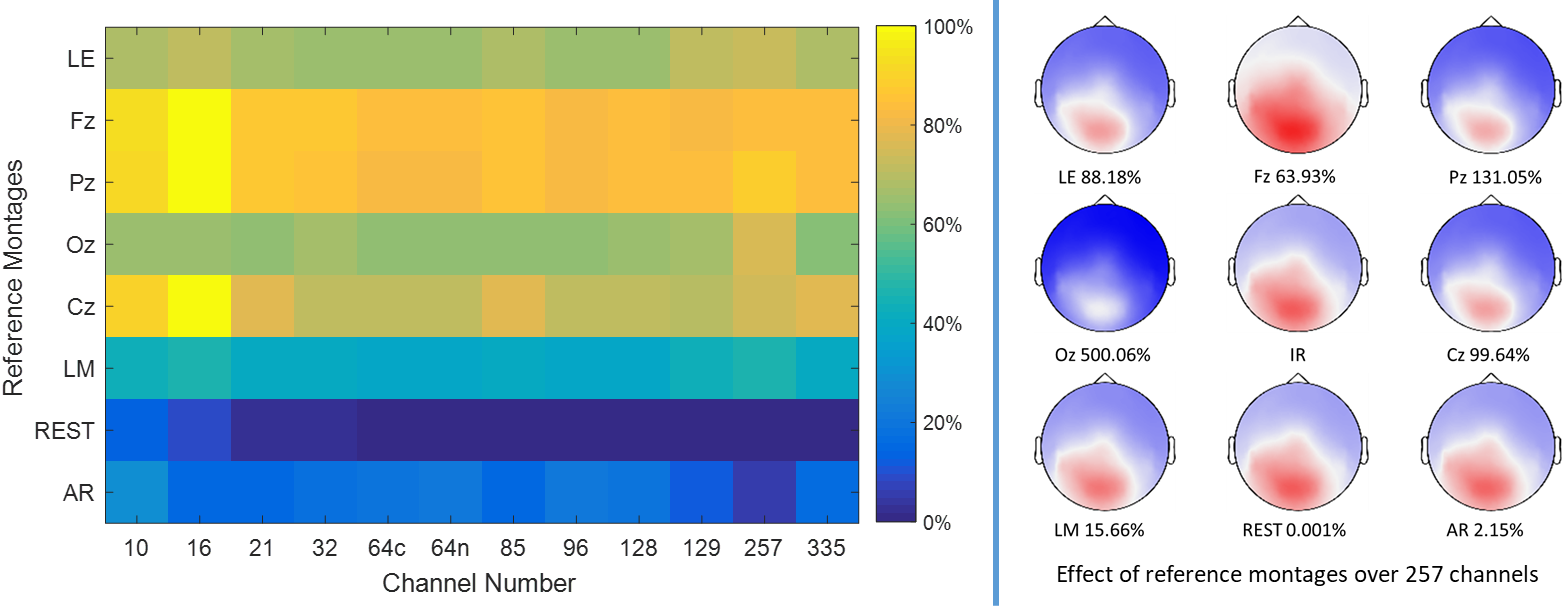
\includegraphics[width=15cm]{pic/JNE/figure3.png}
	\caption{参考模态因素下的电势相对误差,64c和64n分别指的是10-10 c和10-10 n电极分布下的64通道。相对误差RE是逐个激活6407个偶极
	子得到头表电位参考前后相对误差在所有偶极子上的均值;AR和REST关于所有偶极子的标准偏差SD表示在\ref{2:chn}中;所有地形图颜色尺度相同。}
	\label{2:re}
\end{figure}

\subsection{电极数的影响}
因为REST和AR远领先其他参考,从这一节开始重点比较二者,就稀疏阵列和致密阵列来评价电极数的效果。除所有电极(AS)相对误差外还计算部分区域电极相对误差。基于传统地形图拓扑,AS被划分为额叶电极(FS)、颞叶电极(TS)、顶叶电极 (PS) 和枕叶电极(OS)。图\ref{2:chn}中二维电极分布表示如何划分电极区域。由于左右颞叶电极对称,这里只考虑左侧颞叶。因为图\ref{2:chn}的Y轴是$\log_{10}$尺度,不论在所有电极上还是致密阵列的部分电极上,AR具有比REST明显更高的相对误差。 稀疏阵列的部分电极上REST的相对误差在21和32通道时还比AR小很多;10和16通道电极数下,REST的相对误差较大但还比AR要小。这说明REST能在十分稀疏的阵列中取得比AR更好的效果。REST比AR相对误差较小不仅表现在所有电极还表现在部分电极,表明REST不受电极数影响对矫正脑电电位总比AR更好。
AR的相对误差没有随电极数增多线性下降,意味着致密电极阵列未能改善AR,电极数或电极密度对AR来说并不重要。基于物理假设,AR的优势来自大量电极数和头表电极宽泛覆盖\citing{christodoulakis_m_effect_2013},该结果与基于物理假设的共识不一致。REST的标准偏差总比AR的标准偏差小。关于电极数和头表区域的仿真中,REST比AR表现更鲁棒。
\bigskip
\begin{figure}[!ht]
	\centering
	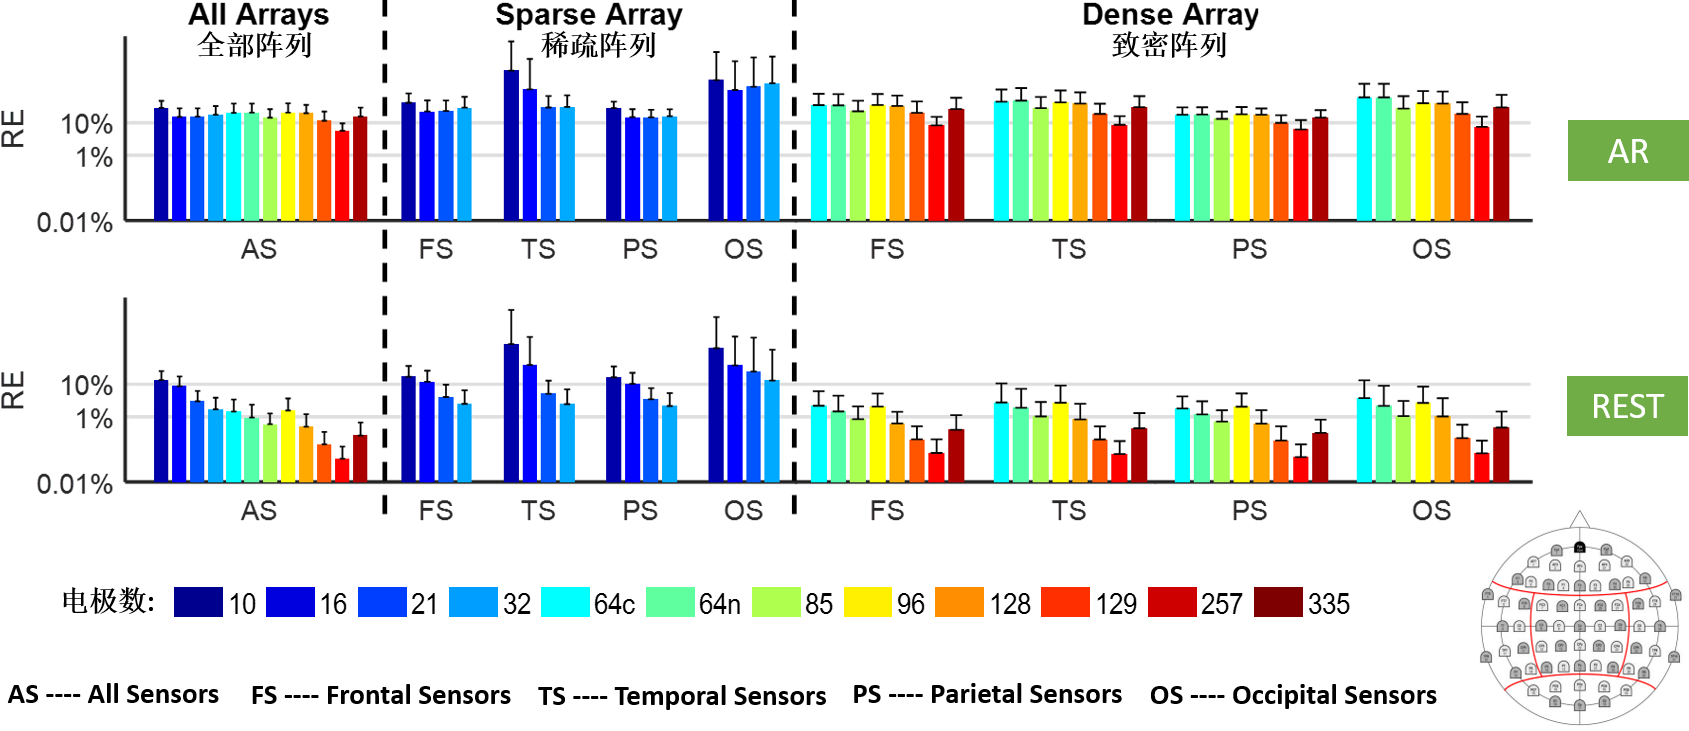
\includegraphics[width=15cm]{pic/JNE/figure4.png}
	\caption{电极数因素下的电位相对误差。所有电极阵列: 10-335,稀疏阵列: ≤32,致密阵列: ≥64; Y轴显示在$\log_{10}$尺度。}
	\label{2:chn}
\end{figure}
\bigskip

\subsection{电极分布的影响}
图\ref{2:layre}表示10-x分布(BP128、BP335)和GSN分布(EGI129、EGI257)间的电位相对误差比较。每种分布都配准在球面或实际头模型表面便于观测每种配置的分布位置。BP128和BP335分别按照10-10 c和10-05系统,二者均只有头皮上表面区域被覆盖。相比,除完全不同的电极放置准则,更多区域如下巴和脖子也被EGI129和EGI257采样。图\ref{2:layre}中关于四种电极配置的相对误差对s REST分别是0.50\%、0.14\%、0.05\%、0.27\%和对s AR分别是19.56\%、11.50\%、5.67\%、15.65\%。显然,相对于10-x分布,GSN分布的REST和AR都具有更低的相对误差。说明宽泛电极覆盖对REST有提升作用,但主要对AR提升较大。BP128与EGI129具有几乎一样多的电极数但电极分布不同,AR的相对误差就从19.56\%下降到11.50\%。但在BP128基础上增加200多电极形成BP335,后者具有十分高的空间采样和致密覆盖却发现AR的相对误差仅从19.56\%略微下降到15.65\%。然而EGI257分布AR的相对误差减少到BP335相对误差的三分之一,但前者仅比后者少大约80个电极。如果用真实头模型取代三层同心球面头模型,以上结果不变。这说明AR的关键是宽泛电极覆盖而非电极数,REST在较多电极数情况下比AR更优。
\begin{figure}[!ht]
	\centering
	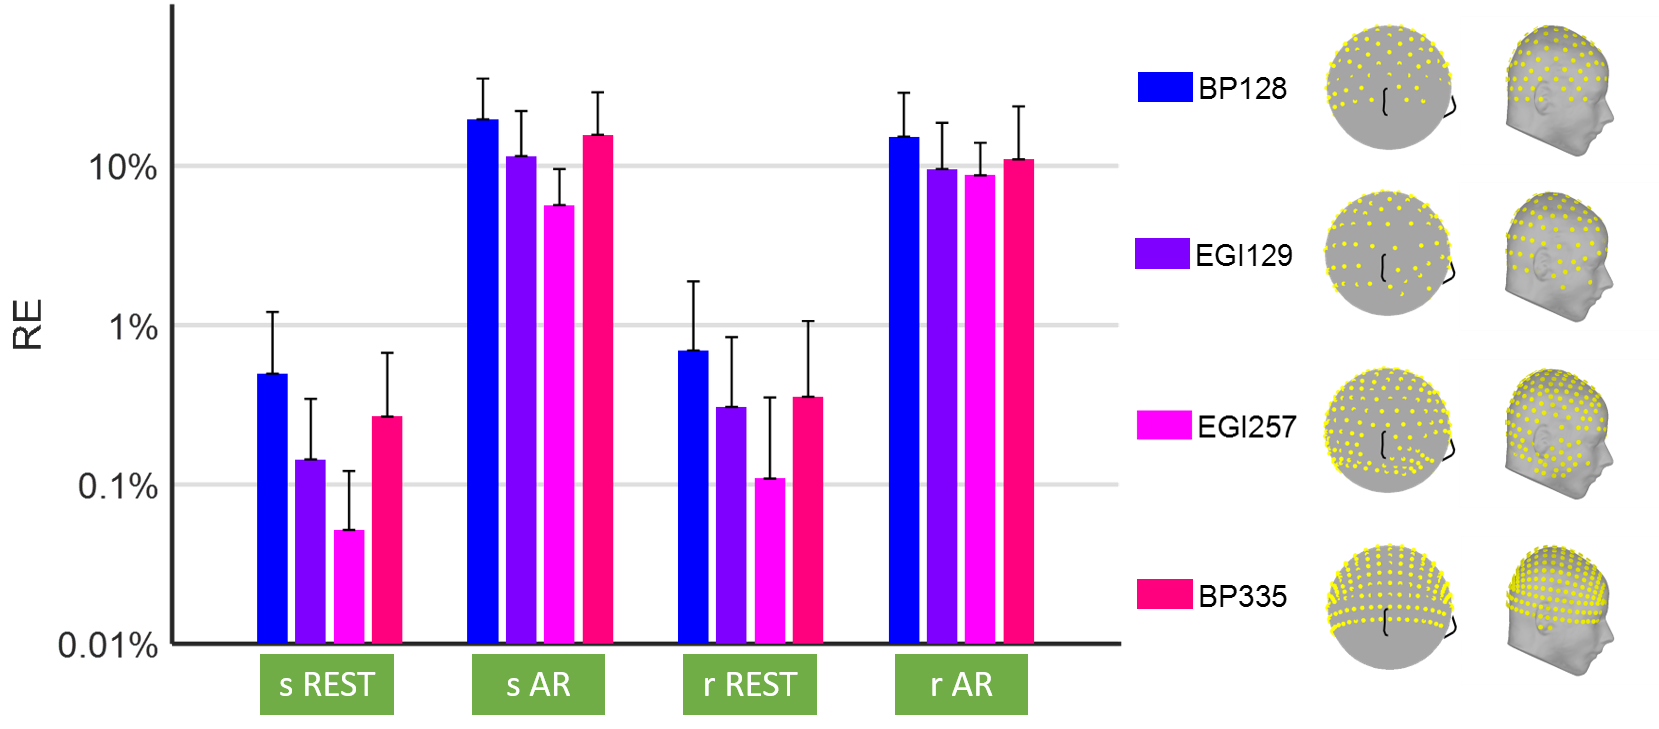
\includegraphics[width=\linewidth]{pic/JNE/figure5.png}
	\caption{电极分布因素下的电位相对误差。 RE显示在$\log_{10}$尺度上,横轴上前缀s和r分别表示球面和真实头模型。BP128和BP335符合10-x分布,EGI129符合GSN分布。头表面黄点代表电极位置。}
	\label{2:layre}
\end{figure}

\subsection{偶极子源位置的影响}
\begin{figure}[h!]
	\centering
	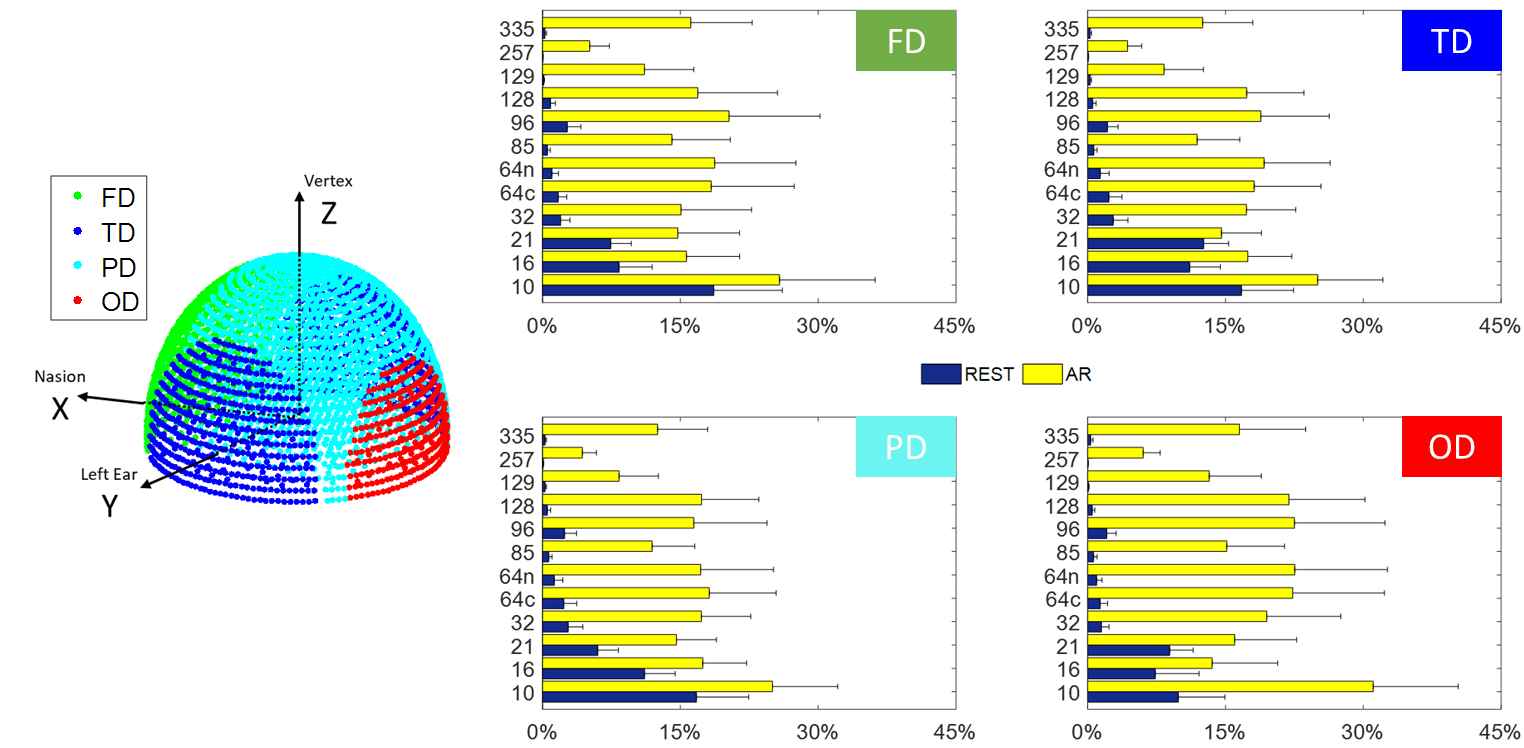
\includegraphics[width=15cm]{pic/JNE/figure6.png}
	\caption{偶极子源位置因素下的电位相对误差。 半球面表示三层同心球面模型下的源空间和坐标。 XYZ轴的方向分别是从圆心朝向鼻根、左耳、上边顶点。}
	\label{2:dip}
\end{figure}
给定电极配置和头模型,脑电电位仍受到偶极子位置影响。将2600个皮层偶极子和1269*3正交栅格偶极子按大脑体素分区划分为四个脑区。图\ref{2:dip}的半球面表示所有偶极子源怎样被划为额叶偶极子(FD)、颞叶偶极子(TD)、顶叶偶极子(PD)和枕叶偶极子(OD)。图\ref{2:dip}的柱状图表示所有电极的电位相对误差但只是由单个感兴趣脑区生成的。FD、TD、PD和OD生成的脑电电位相对误差顺次表示在从左顶端到右下端柱状图中。REST和AR的相对误差分别用蓝色和黄色表示。不论偶极子源分布哪个脑区,REST总能产生比AR更小的相对误差。

\subsection{偶极子源方向的影响}
除了源位置,源活动方向可能对获取脑电电位准确率有较大影响。图\ref{2:orie}表示靠近皮层径向活动的偶极子或体素栅格偶极子沿着XYZ三正交方向其中之一活动产生的脑电电位相对误差。REST和AR的相对误差在X和Y方向上并没有像Z方向上表现出相当大差异,但REST和AR在Y方向比X方向表现出更明显相似性。对于靠近皮层的径向偶极子,REST和AR相对误差的差异程度似乎是XYZ三个方向上差异的折中。该结果可能和电极位置的空间对称性有关。注意到图\ref{2:layout}中如果把二维电极分布转换到球面或如图\ref{2:layre}的三维电极分布,左右电极区域完美对称,前后电极区域对称性很好但不完美,上下电极区域对称性特别差。偶极子源各方向的相对误差相似表明REST能鲁棒地矫正脑电电位。AR在径向和Z方向比XY方向大得多的相对误差可能警示AR受到偶极子源活动方向的制约,可能只适合水平横断面偶极子活动的电位矫正。
\begin{figure}[h!]
	\centering
	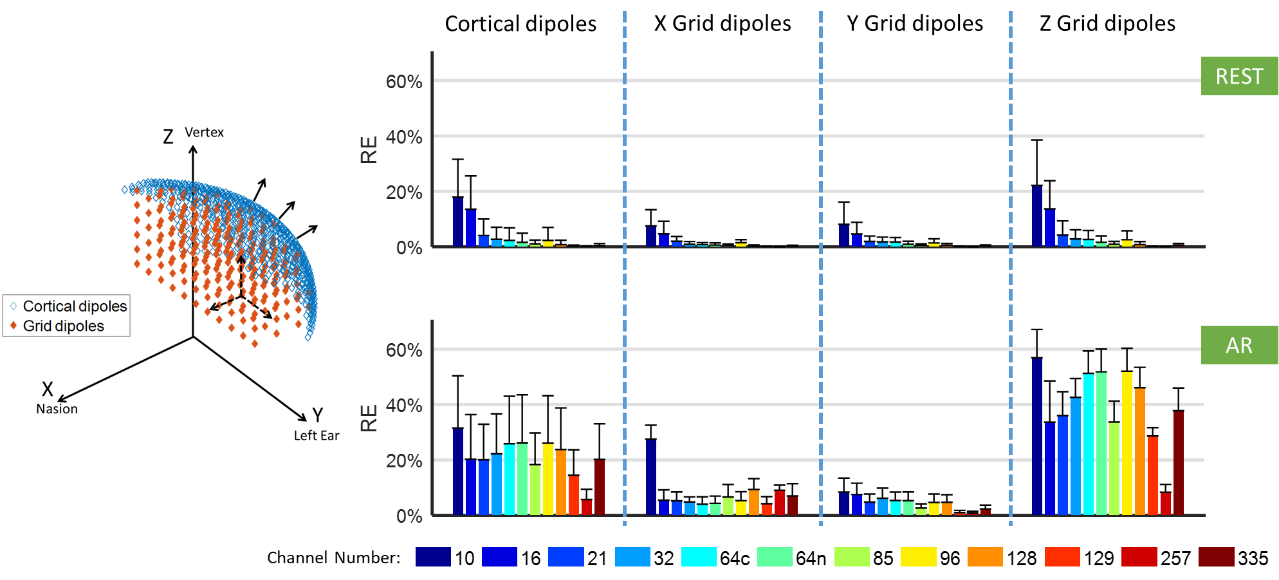
\includegraphics[width=15cm]{pic/JNE/figure7.png}
	\caption{神经源活动方向因素下的电位相对误差。 三维图形是部分偶极子的示例,其中蓝色菱形表示径向垂直于皮层的偶极子,红色菱形表示
	三正交方向的位于栅格顶点的偶极子。}
	\label{2:orie}
\end{figure}

\subsection{传感器电极噪声的影响}
图\ref{2:noise}表示REST和AR对于传感器电极噪声敏感性的比较。没有电极噪声的情况对应于SNR=Inf$\,$dB。从砖红色到蓝色,SNR分别是40、30、20、10、8、4和2dB。相同颜色的标号相连描绘出相对误差随电极数的
变化趋势。显然图\ref{2:noise}A中虚线的间隔比图\ref{2:noise}B的大,A中的虚线比B中低,除了SNR<20dB条件下257通道具有宽泛电极覆盖和SNR$\leq$4dB所有情况时,AR在电极数21、64、96、257比REST好一点。这些结果表明1.REST可能比AR对传感器电极噪声更敏感;2.如果脑电噪声很小,REST还比AR更优;3.通过简单的平均可能起到去噪作用,AR可能适用更高噪声的情形。
\begin{figure}[h!]
	\centering
	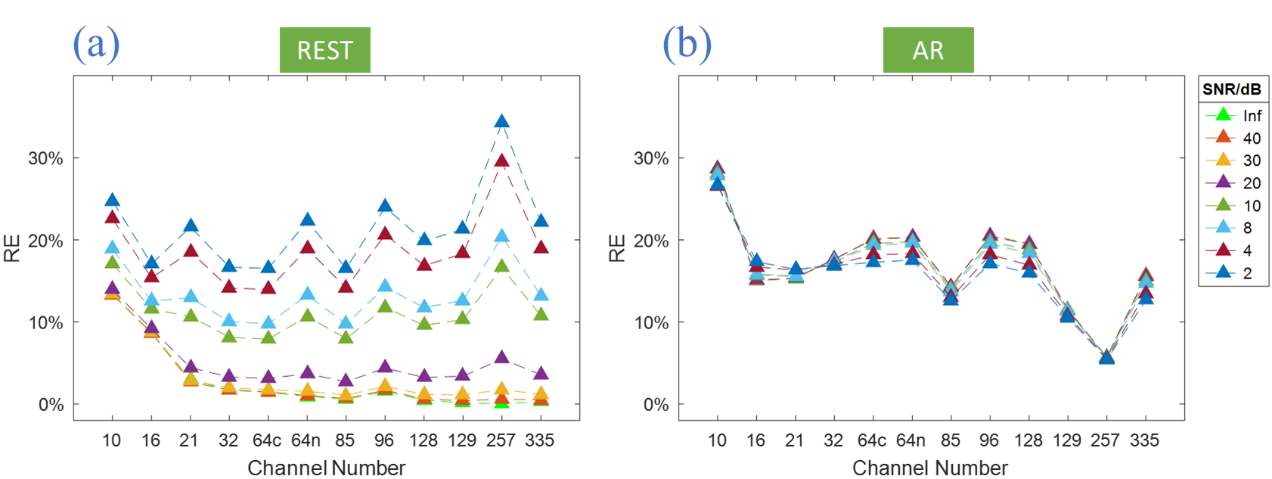
\includegraphics[width=15cm]{pic/JNE/figure8.png}
	\caption{传感器电极噪声因素下的电位相对误差。 不同颜色的标号对应不同的SNR。}
	\label{2:noise}
\end{figure}
\begin{figure}[!ht]
	\centering
	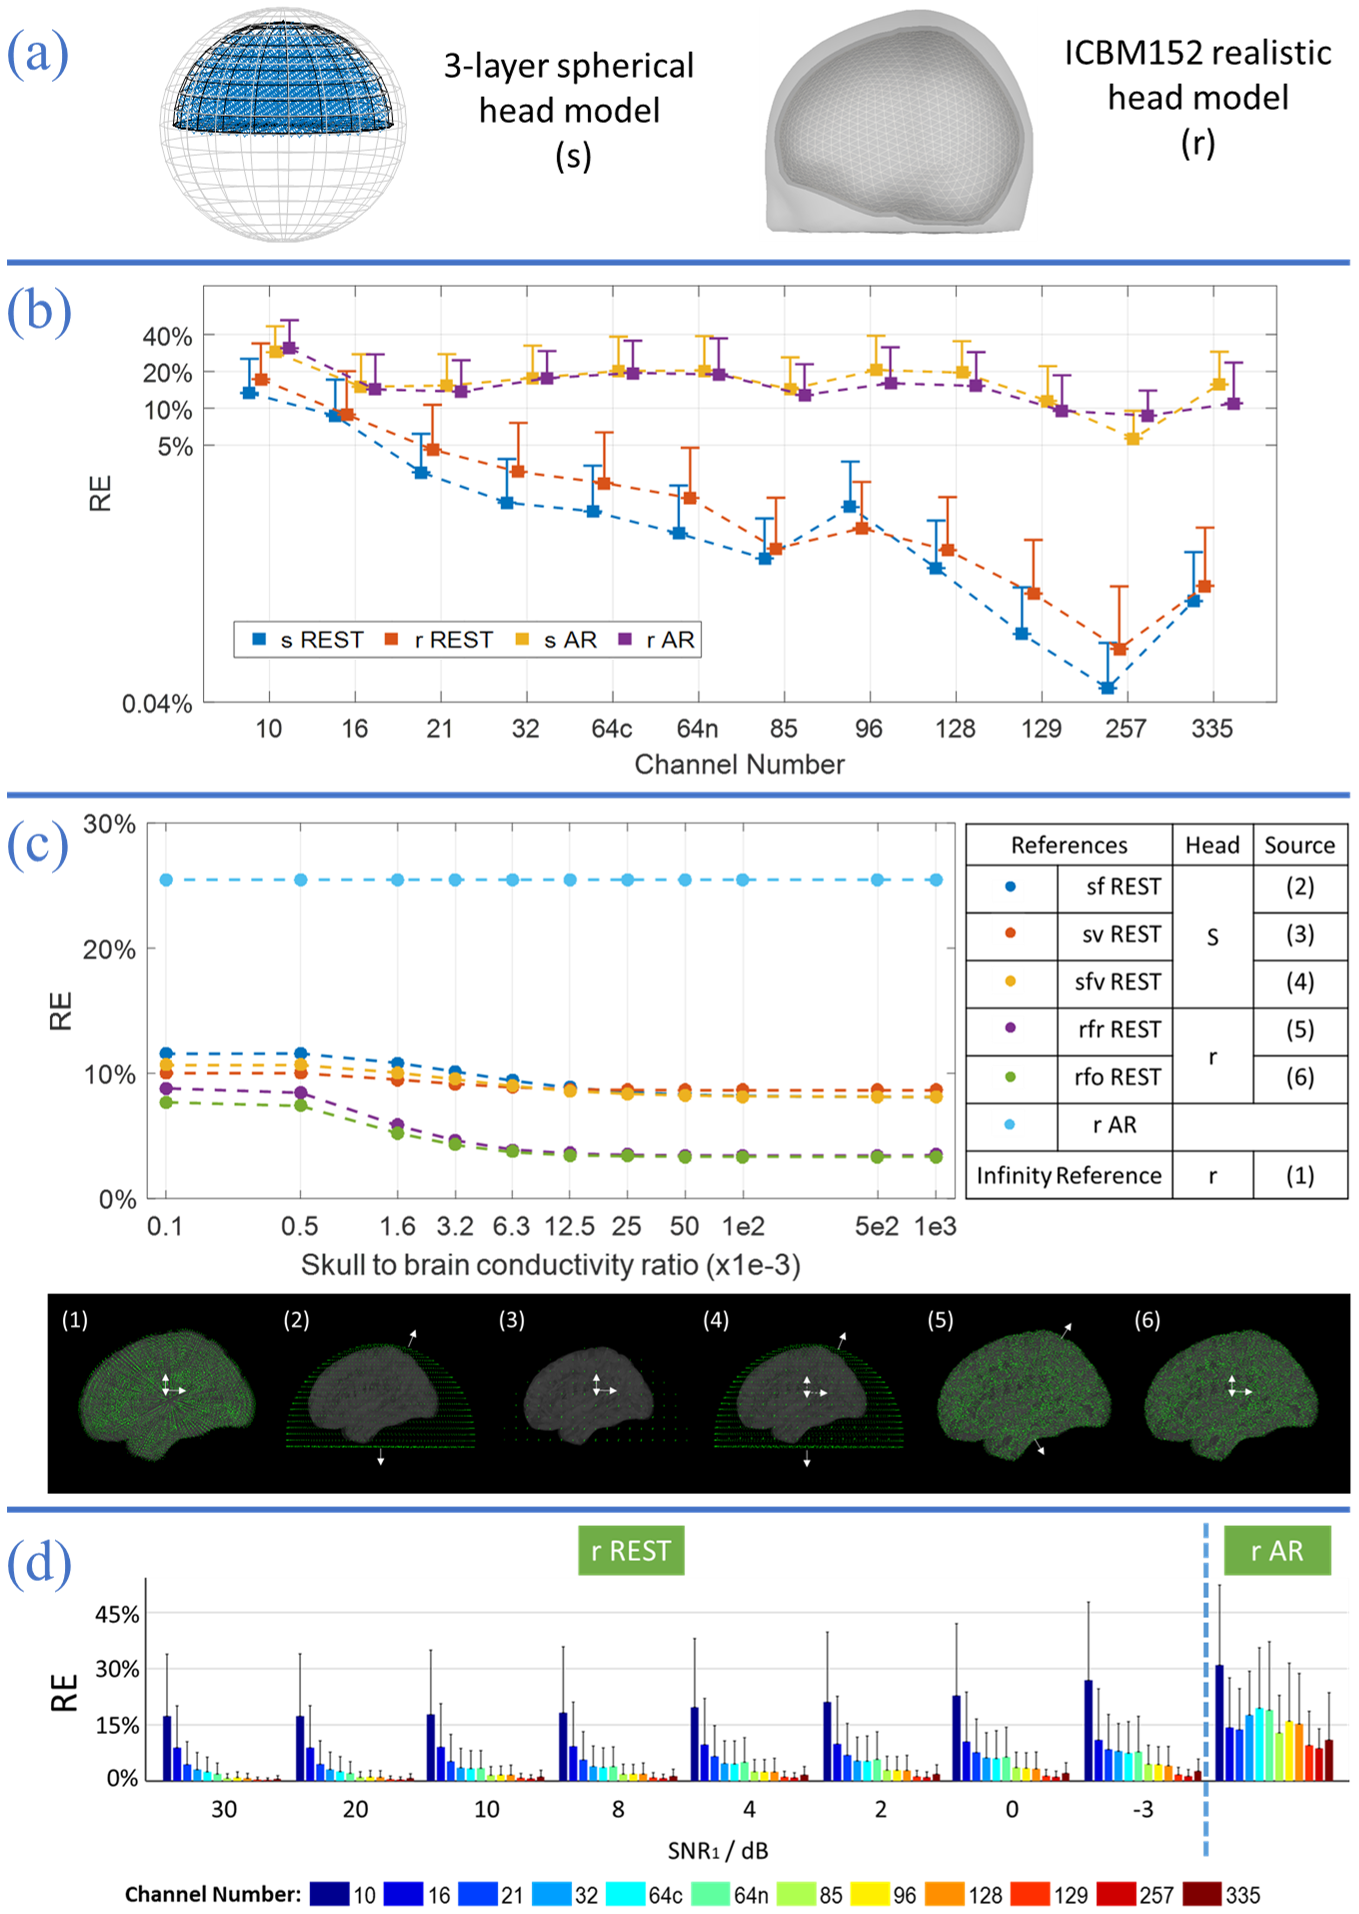
\includegraphics[width=12cm]{pic/JNE/figure9.png}
	\caption{头模型因素的电位相对误差。A.头模型;B.不同头模型下AR和REST的相对误差;C.r\,REST在64\,c电极分布采用与仿真不同的颅骨
	传导率、头形状、源空间作为扰动的结果;黑色条表示6种源配置,白色箭头表示偶极子的方向:(1)17层体素和15765*3正交偶极子;(2)等效分布源层2600个径向皮层偶极子和400个垂直水平断面偶极子;(3)1269*3正交体素偶极子;(4)是(2)和(3)的组合;(5)15002径向皮层偶极子;(6)15002*3正交皮层偶极子。前缀s、r表示头形状,f、v、fv分别表示皮层、体素、皮层组合体素的偶极子,第3个r、o指径向、正交方向;D.对传递矩阵引入噪声作为扰动对r\,REST的影响。}
	\label{2:hm}
\end{figure}
\subsection{头模型的影响}
\label{2:hm-disturb}
图\ref{2:hm}A表示三层同心球模型s和ICBM152实际头模型r,这两种头模型下仿真分析流程相同。基于这两种头模型生成脑电电位条件下REST和AR相对误差比较如图\ref{2:hm}B所示。红色紫色虚线间大间隙证明所有电极数的r\,REST依然比r\,AR相对误差低得多。这表明REST的合理性可能不取决于头形状复杂度。为检查REST是否依赖头形状准确度、颅骨传导率和源空间配置情况,当被试的这三因素值均未知时无穷远参考下的脑电电位使用真实头形状、颅骨相对大脑传导率0.0125、如图\ref{2:hm}C的黑色条中的(1)所示的源配置,但REST重建脑电电位时使用的是各种因素的组合,如头形状可能是球形或真
实的(s, r)、颅骨对大脑传导率设置为(0.0001、0.0005、0.0016、0.0032、0.0063、0.0125、0.025、0.05、0.1、0.5、1),源空间配置如图\ref{2:hm}C中的(2)–(6)所示。 显然,REST比AR的优势可在简单球面头形状、颅骨对大脑传导率为0.0001、源空间配置为(2)–(6)中不同情况都得到保持。REST的相对误差随仿真中对头形状、颅骨脑相对传导率、源空间配置的更好近似而减小。为模拟不精确头模型,引入噪声检查r\,REST受到头模型扰动影响的结果如图\ref{2:hm}D所示。 尽管有两倍(-3dB)的噪声引入到REST的传递矩阵$\mathbf{K}_1$,r\,REST仍比r\,AR误差更小。这些结果表明REST对头模型的扰动不敏感,在使用不精确头模
型时仍保持优势。

\section{讨论}
以前的研究已注意到中立参考估计和电极分布对标准化脑电记录的重要性。最早可追溯到1965年,有研究比较双极、单极、平均参考的性能\citing{osselton_j_w_acquisition_1965};D. Yao提出REST来逼近无穷远参考\citing{yao_method_2001};Q. Liu发现高密度阵列对AR重要,实际头模型对REST很重要\citing{liu_q_estimating_2015};10-20、10-10和10-5系统是基于相对等分头表面电极位置的准则相继拓展出的\citing{jurcak_v_1020_2007}。但还没研究同时考察多种可选的参考模态和各种各样的电极配置。本章全面探究了头表脑电电位如何受到参考模态、电极分布、电极数目、头皮电极区域、偶极子源位置和方向以及电极测量噪声和头模型的影响。

这里发现要用重参考矫正在线记录参考造成的脑电电位高度失真,REST可能是一种比广泛使用的AR更有潜力的参考。对于电极数REST表现出比AR好很多的性能,不仅对全部电极而且对部分头表区域电极亦然。出乎意料的是AR不随电极数增多而改善,更加宽泛的电极覆盖对AR至关重要。这与以前的结果不一致,以前结果认为高密度阵列下AR的使用可能作为金标准\citing{kayser_j_and_tenke_c_e_search_2010,
srinivasan_r_spatial_1998}。无论偶极子源位置在哪,REST都比AR误差更小。相比,AR可能仅适合横断面朝向的偶极子源,但不论偶极子源如何朝向REST都较稳定。对电极测量噪声REST比AR有些敏感,但对一般情况都更优。真实头模型扰动并重复分析表示REST的优势在不太精确的头模型时也能保持。

这些结果可能表明REST能鲁棒地重建脑电电位,但AR受到电极覆盖区域和偶极子源方向的制约。二者的鲜明差异可从它们物理学的理论假设进行解释。AR的假设是容积导体上的电位表面积分为零\citing{schiff_s_j_dangerous_2005,bertrand_theoretical_1985,nunez_electric_2006}。最近研究结果表明真实头表面上积分可能不是零\citing{yao_is_2017},因此头表面均匀采样的零积分假设不再是准确结论。另外,均衡的覆盖不切合实际,如放足够多的电极在面部、脖子和下巴以至于电位积分近似为零,但这正是AR的要求。头表面的下半部分难以如头皮一样做到致密覆盖。还有不均匀脑组织的各向异性传导率使表面电位积分不可能为零。本章AR的结果验证了D. Yao的讨论\citing{yao_is_2017}。相比,REST用到等效源的物理事实作为内在桥梁,变换一种脑电参考到另一个。尽管实际神经源的求解不唯一,任何非无穷远参考下的脑电电位可借助等效源的唯一性来近似重建。实现REST最简单的方式是基于具有记录参考的传递矩阵用最小模解逆问题,再进行正演计算\citing{dong_l_matlab_2017}。本章研究扩展
了Q. Liu\citing{liu_q_estimating_2015}的工作,主要采用较好构造的三层同心球头模型\citing{yao_method_2001},结合各种参考模态和更多种电极配置。本章结果与Q. Liu的不同体现在以下三个方面:首先,AR的主要因素是电极分布是否满足宽泛覆盖而非电极数目;其次,REST比AR的优势存在于本章研究的所有电极数和电极分布;尽管REST依赖于头模型但其优势对头模型扰动不敏感。这是首个全面探讨参考模态和电极分布如何影响脑电记录准确性的研究。这些结果可能为神经认知和临床定量脑电分析中使用最优参考提供建议。然而,本研究还存在一些不足。尽管采用边界元法\citing{gramfort_a_openmeeg_2010}建立实际的头模型,有限元法或者有限差分法\citing{hallez_h_et_al_review_2007}提供比边界元法获得更准确颅骨传导率的可能性\citing{akhtari_m_conductivities_2002,ziegler_e_finite-element_2014}。 此外,本章脑电电位的准确性指的是电位相对误差,这种误差是基于容积传导的瞬时效应。然而,时空分析、时频分析甚至源成像也可能受到参考模态和电极分布的影响 \citing{nunez_p_l_eeg_1997,yao_d_comparative_2005,essl_m_and_rappelsberger_p_eeg_1998,marzetti_l_use_2007,lantz_g_epileptic_2003,tenke_c_and_kayser_j_reference-free_2005,pivik_r_t_guidelines_1993,hagemann_d_quest_2001}。
\section{本章小结}
本章系统研究了参考模态和电极配置因素如何影响脑电电势的准确性,发现无穷远参考和平均参考是两种有效的重参考方法,优于单极参考或者连接耳。从电极数量、头表区域、电极分布、偶极子源的位置与方向以及电极噪声和容积传导头模型角度进行比较研究,发现零参考比平均参考更鲁棒地矫正失真的电势,平均参考的性能与电极数并无关系但受电极覆盖范围及偶极子源方向的制约。